\documentclass[12pt,a4paper]{ctexart}
\usepackage[utf8]{inputenc}
\usepackage{ctex}
\usepackage{amsmath}
\usepackage{geometry}
\usepackage{booktabs}
\usepackage{hyperref}
\usepackage{graphicx} 
\usepackage{listings} 
\usepackage{xcolor}
\usepackage{booktabs}

% 页面边距设置
\geometry{left=2.5cm,right=2.5cm,top=2.5cm,bottom=2.5cm}

\lstset{
    language=C++,
    basicstyle=\ttfamily\small,
    keywordstyle=\color{blue},
    commentstyle=\color{gray},
    stringstyle=\color{orange},
    numbers=left,
    numberstyle=\tiny\color{gray},
    breaklines=true,
    frame=single,
    backgroundcolor=\color{lightgray!10},
    xleftmargin=1em,
    showstringspaces=false
}

\title{\textbf{实验报告：CPU 架构相关编程}}
\author{
    姓名：王绅 \quad 学号：2412780 \\
    专业：计算机科学与技术 \quad 年级：大二
}
\date{\today}

\begin{document}

\maketitle

\section{源码项目链接}

\begin{itemize}
    \item \textbf{项目地址}：\url{[https://github.com/wshen3500-stack/bingxingchengxusheji]}
\end{itemize}

\section{实验平台配置}
\begin{itemize}
    \item \textbf{操作系统}：windows
    \item \textbf{开发工具}：Visual Studio Code (VS Code) 
    \item \textbf{编译器}：GCC (g++)，支持 C++11/17 标准
    \item \textbf{硬件平台}：x86\_64 架构
\end{itemize}

\section{程序设计思路与核心代码展示}
本实验旨在探索 Cache 命中率和指令级并行（ILP）对程序性能的决定性影响 。研究cache的局限性和指令级并行能力

\subsection{一：矩阵-向量乘法优化 (Cache 友好性)}
计算 $n \times n$ 矩阵与向量的内积（$n=10000$）。

\subsubsection{设计思路}
C/C++ 中二维数组按行优先  存储 。平凡算法 (\texttt{1-a.cpp}) 采用外层循环遍历列、内层遍历行，这种访问模式违背了数据的物理存储规律，导致内存读取地址发生大跨度的跳跃，导致内存访问不连续，产生严重的跨步访问，极大增加了 Cache Miss。
优化算法 (\texttt{1-b.cpp}) 通过交换循环顺序，外层循环行，内层循环列。实现了内存的连续读取。极大提高了内存总线的实际有效带宽。

\subsubsection{关键代码对比}
\begin{lstlisting}[caption={平凡算法中的跨步访问 (1-a.cpp)}]
// 外层循环列，内层循环行
for (int a = 0; a < Max; a++) {
    for (int b = 0; b < Max; b++) {
        y[a] += data[b][a] * x[b];
    }
}
\end{lstlisting}

\begin{lstlisting}[caption={优化算法中的连续访问 (1-b.cpp)}]
// 外层循环行，内层循环列
for (int a = 0; a < Max; a++) {
    for (int b = 0; b < Max; b++) {
        y[b] += data[a][b] * x[a];
    }
}
\end{lstlisting}

\subsection{问题二：$n$ 个数累加优化 (超标量与 ILP)}
对规模为 $500,000$ 的浮点数组求和。
\subsubsection{设计思路}
平凡算法 (\texttt{2-b.cpp}) 采用单一累加器，存在“写后读”数据依赖，导致cpu的其他算术逻辑单元属于闲置的状态，限制了流水线吞吐 。
优化算法 (\texttt{2-a.cpp}) 采用 4 路循环展开与独立累加器，每次循环同步处理四个数组元素的累加，打破了依赖链，充分利用超标量 CPU 的多个执行单元 。

\subsubsection{关键代码展示}
\begin{lstlisting}[caption={4路超标量累加优化 (2-a.cpp)}]
// 使用4个独立寄存器打破数据依赖链
double sum0 = 0.0, sum1 = 0.0, sum2 = 0.0, sum3 = 0.0;
for (int j = 0; j <= Max - 4; j += 4) {
    sum0 += arr[j];
    sum1 += arr[j+1];
    sum2 += arr[j+2];
    sum3 += arr[j+3];
}
final_result = sum0 + sum1 + sum2 + sum3;
\end{lstlisting}

\section{实验方案设计}
\begin{itemize}
    \item \textbf{测试数据}：采用人为设计的规律值（如 \texttt{i * 1.5}）初始化，确保结果可验证 。
    \item \textbf{重复实验}：设置 \texttt{rounds = 1000}，通过多次迭代取平均耗时，以缓解背景进程调度带来的随机误差 。
    \item \textbf{防止过度优化}：将结果赋值给全局或 \texttt{volatile} 变量，防止编译器由于结果未被使用而剔除整个循环 。
\end{itemize}

\section{实验结果呈现及分析}

\subsection{性能结果统计}

\begin{table}[htbp]
    \centering
    \begin{tabular}{cccc}
        \toprule
        \textbf{实验项目} & \textbf{算法版本} & \textbf{平均耗时 (ms)} & \textbf{性能加速比} \\
        \midrule
        矩阵-向量内积 & 平凡算法 (\texttt{1-a}) & [652.193] & 1.00 \\
                      & Cache 优化 (\texttt{1-b}) & [230.989] & [2.08]x \\
        \midrule
        数组累加求和 & 平凡链式 (\texttt{2-a}) & [2.494] & 1.00 \\
                      & 超标量优化 (\texttt{2-b}) & [0.686] & [3.64]x \\
        \bottomrule
    \end{tabular}
    \caption{实验性能数据对比记录}
\end{table}

\subsection{执行结果}


\begin{figure}[htbp]
    \centering
   
     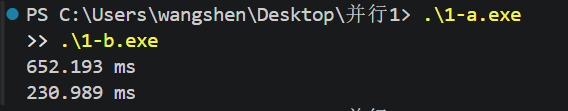
\includegraphics[width=0.8\textwidth]{result1.png} 

    \caption{问题一：Cache 优化前后的性能差异截图}
\end{figure}

\begin{figure}[htbp]
    \centering
    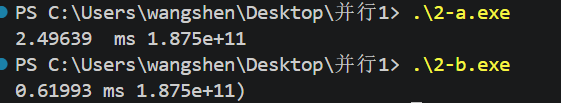
\includegraphics[width=0.8\textwidth]{result2.png}
    
    \caption{问题二：超标量优化前后的性能差异截图}
\end{figure}

\section{结论分析}
1. \textbf{局部性原理}：实验一证明了访存模式对性能的巨大影响。连续访存能使数据留在 L1/L2 Cache 中，极大地减少了由于跨步访问引起的总线等待。
2. \textbf{流水线并行}：实验二展示了超标量 CPU 的潜力。通过多路累加，我们手动打破了指令流中的依赖，让处理器的多个 ALU 能够并行工作，从而在计算密集型任务中获得显著加速。



\end{document}